% Options for packages loaded elsewhere
\PassOptionsToPackage{unicode}{hyperref}
\PassOptionsToPackage{hyphens}{url}
%
\documentclass[
  man]{apa6}
\usepackage{amsmath,amssymb}
\usepackage{iftex}
\ifPDFTeX
  \usepackage[T1]{fontenc}
  \usepackage[utf8]{inputenc}
  \usepackage{textcomp} % provide euro and other symbols
\else % if luatex or xetex
  \usepackage{unicode-math} % this also loads fontspec
  \defaultfontfeatures{Scale=MatchLowercase}
  \defaultfontfeatures[\rmfamily]{Ligatures=TeX,Scale=1}
\fi
\usepackage{lmodern}
\ifPDFTeX\else
  % xetex/luatex font selection
\fi
% Use upquote if available, for straight quotes in verbatim environments
\IfFileExists{upquote.sty}{\usepackage{upquote}}{}
\IfFileExists{microtype.sty}{% use microtype if available
  \usepackage[]{microtype}
  \UseMicrotypeSet[protrusion]{basicmath} % disable protrusion for tt fonts
}{}
\makeatletter
\@ifundefined{KOMAClassName}{% if non-KOMA class
  \IfFileExists{parskip.sty}{%
    \usepackage{parskip}
  }{% else
    \setlength{\parindent}{0pt}
    \setlength{\parskip}{6pt plus 2pt minus 1pt}}
}{% if KOMA class
  \KOMAoptions{parskip=half}}
\makeatother
\usepackage{xcolor}
\usepackage{graphicx}
\makeatletter
\def\maxwidth{\ifdim\Gin@nat@width>\linewidth\linewidth\else\Gin@nat@width\fi}
\def\maxheight{\ifdim\Gin@nat@height>\textheight\textheight\else\Gin@nat@height\fi}
\makeatother
% Scale images if necessary, so that they will not overflow the page
% margins by default, and it is still possible to overwrite the defaults
% using explicit options in \includegraphics[width, height, ...]{}
\setkeys{Gin}{width=\maxwidth,height=\maxheight,keepaspectratio}
% Set default figure placement to htbp
\makeatletter
\def\fps@figure{htbp}
\makeatother
\setlength{\emergencystretch}{3em} % prevent overfull lines
\providecommand{\tightlist}{%
  \setlength{\itemsep}{0pt}\setlength{\parskip}{0pt}}
\setcounter{secnumdepth}{-\maxdimen} % remove section numbering
% Make \paragraph and \subparagraph free-standing
\makeatletter
\ifx\paragraph\undefined\else
  \let\oldparagraph\paragraph
  \renewcommand{\paragraph}{
    \@ifstar
      \xxxParagraphStar
      \xxxParagraphNoStar
  }
  \newcommand{\xxxParagraphStar}[1]{\oldparagraph*{#1}\mbox{}}
  \newcommand{\xxxParagraphNoStar}[1]{\oldparagraph{#1}\mbox{}}
\fi
\ifx\subparagraph\undefined\else
  \let\oldsubparagraph\subparagraph
  \renewcommand{\subparagraph}{
    \@ifstar
      \xxxSubParagraphStar
      \xxxSubParagraphNoStar
  }
  \newcommand{\xxxSubParagraphStar}[1]{\oldsubparagraph*{#1}\mbox{}}
  \newcommand{\xxxSubParagraphNoStar}[1]{\oldsubparagraph{#1}\mbox{}}
\fi
\makeatother
% definitions for citeproc citations
\NewDocumentCommand\citeproctext{}{}
\NewDocumentCommand\citeproc{mm}{%
  \begingroup\def\citeproctext{#2}\cite{#1}\endgroup}
\makeatletter
 % allow citations to break across lines
 \let\@cite@ofmt\@firstofone
 % avoid brackets around text for \cite:
 \def\@biblabel#1{}
 \def\@cite#1#2{{#1\if@tempswa , #2\fi}}
\makeatother
\newlength{\cslhangindent}
\setlength{\cslhangindent}{1.5em}
\newlength{\csllabelwidth}
\setlength{\csllabelwidth}{3em}
\newenvironment{CSLReferences}[2] % #1 hanging-indent, #2 entry-spacing
 {\begin{list}{}{%
  \setlength{\itemindent}{0pt}
  \setlength{\leftmargin}{0pt}
  \setlength{\parsep}{0pt}
  % turn on hanging indent if param 1 is 1
  \ifodd #1
   \setlength{\leftmargin}{\cslhangindent}
   \setlength{\itemindent}{-1\cslhangindent}
  \fi
  % set entry spacing
  \setlength{\itemsep}{#2\baselineskip}}}
 {\end{list}}
\usepackage{calc}
\newcommand{\CSLBlock}[1]{\hfill\break\parbox[t]{\linewidth}{\strut\ignorespaces#1\strut}}
\newcommand{\CSLLeftMargin}[1]{\parbox[t]{\csllabelwidth}{\strut#1\strut}}
\newcommand{\CSLRightInline}[1]{\parbox[t]{\linewidth - \csllabelwidth}{\strut#1\strut}}
\newcommand{\CSLIndent}[1]{\hspace{\cslhangindent}#1}
\ifLuaTeX
\usepackage[bidi=basic]{babel}
\else
\usepackage[bidi=default]{babel}
\fi
\babelprovide[main,import]{english}
% get rid of language-specific shorthands (see #6817):
\let\LanguageShortHands\languageshorthands
\def\languageshorthands#1{}
% Manuscript styling
\usepackage{upgreek}
\captionsetup{font=singlespacing,justification=justified}

% Table formatting
\usepackage{longtable}
\usepackage{lscape}
% \usepackage[counterclockwise]{rotating}   % Landscape page setup for large tables
\usepackage{multirow}		% Table styling
\usepackage{tabularx}		% Control Column width
\usepackage[flushleft]{threeparttable}	% Allows for three part tables with a specified notes section
\usepackage{threeparttablex}            % Lets threeparttable work with longtable

% Create new environments so endfloat can handle them
% \newenvironment{ltable}
%   {\begin{landscape}\centering\begin{threeparttable}}
%   {\end{threeparttable}\end{landscape}}
\newenvironment{lltable}{\begin{landscape}\centering\begin{ThreePartTable}}{\end{ThreePartTable}\end{landscape}}

% Enables adjusting longtable caption width to table width
% Solution found at http://golatex.de/longtable-mit-caption-so-breit-wie-die-tabelle-t15767.html
\makeatletter
\newcommand\LastLTentrywidth{1em}
\newlength\longtablewidth
\setlength{\longtablewidth}{1in}
\newcommand{\getlongtablewidth}{\begingroup \ifcsname LT@\roman{LT@tables}\endcsname \global\longtablewidth=0pt \renewcommand{\LT@entry}[2]{\global\advance\longtablewidth by ##2\relax\gdef\LastLTentrywidth{##2}}\@nameuse{LT@\roman{LT@tables}} \fi \endgroup}

% \setlength{\parindent}{0.5in}
% \setlength{\parskip}{0pt plus 0pt minus 0pt}

% Overwrite redefinition of paragraph and subparagraph by the default LaTeX template
% See https://github.com/crsh/papaja/issues/292
\makeatletter
\renewcommand{\paragraph}{\@startsection{paragraph}{4}{\parindent}%
  {0\baselineskip \@plus 0.2ex \@minus 0.2ex}%
  {-1em}%
  {\normalfont\normalsize\bfseries\itshape\typesectitle}}

\renewcommand{\subparagraph}[1]{\@startsection{subparagraph}{5}{1em}%
  {0\baselineskip \@plus 0.2ex \@minus 0.2ex}%
  {-\z@\relax}%
  {\normalfont\normalsize\itshape\hspace{\parindent}{#1}\textit{\addperi}}{\relax}}
\makeatother

\makeatletter
\usepackage{etoolbox}
\patchcmd{\maketitle}
  {\section{\normalfont\normalsize\abstractname}}
  {\section*{\normalfont\normalsize\abstractname}}
  {}{\typeout{Failed to patch abstract.}}
\patchcmd{\maketitle}
  {\section{\protect\normalfont{\@title}}}
  {\section*{\protect\normalfont{\@title}}}
  {}{\typeout{Failed to patch title.}}
\makeatother

\usepackage{xpatch}
\makeatletter
\xapptocmd\appendix
  {\xapptocmd\section
    {\addcontentsline{toc}{section}{\appendixname\ifoneappendix\else~\theappendix\fi: #1}}
    {}{\InnerPatchFailed}%
  }
{}{\PatchFailed}
\makeatother
\keywords{graphical representation, iconicity, analogy, symbol, communication, emerging literacy\newline\indent Word count: Child Development Max 40 pages // PNAS 1,500–2,000 words}
\DeclareDelayedFloatFlavor{ThreePartTable}{table}
\DeclareDelayedFloatFlavor{lltable}{table}
\DeclareDelayedFloatFlavor*{longtable}{table}
\makeatletter
\renewcommand{\efloat@iwrite}[1]{\immediate\expandafter\protected@write\csname efloat@post#1\endcsname{}}
\makeatother
\usepackage{lineno}

\linenumbers
\usepackage{csquotes}
\ifLuaTeX
  \usepackage{selnolig}  % disable illegal ligatures
\fi
\usepackage{bookmark}
\IfFileExists{xurl.sty}{\usepackage{xurl}}{} % add URL line breaks if available
\urlstyle{same}
\hypersetup{
  pdftitle={Young children's spontaneous comprehension of symbol-object-relationships in the graphic domain},
  pdfauthor={Gregor Kachel1, Daniel Haun2, \& Manuel Bohn1},
  pdflang={en-EN},
  pdfkeywords={graphical representation, iconicity, analogy, symbol, communication, emerging literacy},
  hidelinks,
  pdfcreator={LaTeX via pandoc}}

\title{Young children's spontaneous comprehension of symbol-object-relationships in the graphic domain}
\author{Gregor Kachel\textsuperscript{1}, Daniel Haun\textsuperscript{2}, \& Manuel Bohn\textsuperscript{1}}
\date{}


\shorttitle{Comprehension of symbol-object-relationships}

\authornote{

\emph{Ethics, consent and conflict of interest}: This study confirms with recognized standards (e.g.~the Declaration of Helsinki) and was approved by an internal ethics committee at the Max-Planck-Institute for Evolutionary Anthropology. Informed consent has been obtained from all participants. The authors declare no conflict of interest.

\emph{Acknowledgments}: We are thankful to Susanne Mauritz for her help in the organization of the study and to Valerie Jurgenson and Cynthia Pones for help with data collection. We would like to thank Anne Deiglmayr for hosting this project in her research group and for her continuous support. Finally, we are very thankful to all parents and children participating in the study. Gregor Kachel was supported by the German Research Foundation (Deutsche Forschungsgemeinschaft) under project number 429220405.

Correspondence concerning this article should be addressed to Gregor Kachel, Dittrichring 5-7, 04109 Leipzig. E-mail: \href{mailto:gregor.kachel@uni-leipzig.de}{\nolinkurl{gregor.kachel@uni-leipzig.de}}

}

\affiliation{\vspace{0.5cm}\textsuperscript{1} Leuphana University\\\textsuperscript{2} Max-Planck-Institute for Evolutionary Anthropology}

\abstract{%
Lorem ipsum dolor sit amet, consetetur sadipscing elitr, sed diam nonumy eirmod tempor invidunt ut labore et dolore magna aliquyam erat, sed diam voluptua. At vero eos et accusam et justo duo dolores et ea rebum. Stet clita kasd gubergren, no sea takimata sanctus est Lorem ipsum dolor sit amet. Lorem ipsum dolor sit amet, consetetur sadipscing elitr, sed diam nonumy eirmod tempor invidunt ut labore et dolore magna aliquyam erat, sed diam voluptua. !Abstract must be less then 120words!
}



\begin{document}
\maketitle

\section{Introduction}\label{introduction}

Lorem ipsum dolor sit amet, consetetur sadipscing elitr, sed diam nonumy eirmod tempor invidunt ut labore et dolore magna aliquyam erat, sed diam voluptua. At vero eos et accusam et justo duo dolores et ea rebum. Stet clita kasd gubergren, no sea takimata sanctus est Lorem ipsum dolor sit amet. Lorem ipsum dolor sit amet, consetetur sadipscing elitr, sed diam nonumy eirmod tempor invidunt ut labore et dolore magna aliquyam erat, sed diam voluptua. At vero eos et accusam et justo duo dolores et ea rebum. Stet clita kasd gubergren, no sea takimata sanctus est Lorem ipsum dolor sit amet.

\emph{General notes Citing stuff}. You have to make sure that the respective reference in included in the bib-file. I would also suggest to have two additional folders in the root, namely (1) papers to cite - where we can dumb pdfs, and (2) papers\_cited. Whenever you are adding a new reference please put the citation in bibtex, name the pdf accorind to the bibtext id and add the pdf to the papers\_cited folder. And this is how to cite something in markdown: Preschoolers invent and comprehend iconic gestures spontaneously (Bohn, Kachel, \& Tomasello, 2019).

\emph{Children's understanding of graphical representations}. Lorem ipsum dolor sit amet, consetetur sadipscing elitr, sed diam nonumy eirmod tempor invidunt ut labore et dolore magna aliquyam erat, sed diam voluptua. At vero eos et accusam et justo duo dolores et ea rebum. Stet clita kasd gubergren, no sea takimata sanctus est Lorem ipsum dolor sit amet. Lorem ipsum dolor sit amet, consetetur sadipscing elitr, sed diam nonumy eirmod tempor invidunt ut labore et dolore magna aliquyam erat, sed diam voluptua. At vero eos et accusam et justo duo dolores et ea rebum. Stet clita kasd gubergren, no sea takimata sanctus est Lorem ipsum dolor sit amet.

\emph{This Paper}. Lorem ipsum dolor sit amet, consetetur sadipscing elitr, sed diam nonumy eirmod tempor invidunt ut labore et dolore magna aliquyam erat, sed diam voluptua. At vero eos et accusam et justo duo dolores et ea rebum. Stet clita kasd gubergren, no sea takimata sanctus est Lorem ipsum dolor sit amet. Lorem ipsum dolor sit amet, consetetur sadipscing elitr, sed diam nonumy eirmod tempor invidunt ut labore et dolore magna aliquyam erat, sed diam voluptua. At vero eos et accusam et justo duo dolores et ea rebum. Stet clita kasd gubergren, no sea takimata sanctus est Lorem ipsum dolor sit amet. For the first time, the studies contributing to this paper investigate children's understanding of xxx.

\emph{Hypotheses}. Lorem ipsum dolor sit amet, consetetur sadipscing elitr, sed diam nonumy eirmod tempor invidunt ut labore et dolore magna aliquyam erat, sed diam voluptua. At vero eos et accusam et justo duo dolores et ea rebum. Stet clita kasd gubergren, no sea takimata sanctus est Lorem ipsum dolor sit amet. Lorem ipsum dolor sit amet, consetetur sadipscing elitr, sed diam nonumy eirmod tempor invidunt ut labore et dolore magna aliquyam erat, sed diam voluptua. At vero eos et accusam et justo duo dolores et ea rebum. Stet clita kasd gubergren, no sea takimata sanctus est Lorem ipsum dolor sit amet.

\section{Methods}\label{methods}

We report how we determined our sample size, all data exclusions, all manipulations, and all measures in the study (Simmons, Nelson, \& Simonsohn, 2012). Supplementary materials document all pilots that were run and the specific conclusions we drew from them during the development of the study. Both supplements and main article are fully reproducible manuscripts (Aust \& Barth, 2022) providing all data and analyses.

\subsection{Participants}\label{participants}

\subsection{Procedure and Setup}\label{procedure-and-setup}

Children were visited in-person at their daycares. Daycares provided a separate room where experimenters (E) and children watched the presentation of a picture-book like hiding game on screen while sitting at their side.

\emph{Familiarization}. E introduced an agent, namely a cartoon monkey, and familiarized children with the framing of the task. The monkey placed two small cups at the bottom of the screen. Next, the cups were lifted and the monkey dropped a banana under one of them. The cups were lowered again to hide the banana. Hence, children saw an item being hidden in plain sight and were solely required to remember its place for a minimal amount of time before being asked ``Where is the banana?''. Children were required to point at the correct hiding place. In the familiarization phase, children received immediate feedback from the experimenter (``Well done!'' / ``hmm, lets go again!'') while the hiding place of the banana was revealed. Children are expected to succeed in at least 4 familiarization trials in a row in order to move to the main test. Familiarization would continue for a minimum of four and a maximum of eight trials. The familiarization ensured that all participants were familiar with the aim of the game and that E was able to read participants' responses.

\emph{Test phase}.The main phase of the study commenced with E announcing that the cartoon character had an idea for a new game. E explains that they must not see where the banana is hidden. The hiding sequence is identical to the familiarization phase, however the placement of the banana is covered by a wood fence over the lower half of the screen. Next, the monkey holds up geometric shape, namely a circle in the \emph{marker condition} and an equilateral triangle in the \emph{arrow condition}. E narrates ``Coco is going to help you find the banana. In the arrow condition, the monkey places the triangle in a central position pointing to either the left or right target. In the marker condition, the monkey places the circle directly on the left or right target. After the placement, children are asked''where is the banana?{}``. The hiding place is not revealed and children do not receive feedback in test trials. E acknowledges their choices by thanking them in a neutral tone and moves on to the next trial.

Except for the geometric shapes and their placement, the presentations in both conditions were identical. A single trial lasted 20 to 30 seconds. Children were presented with a maximum of 16 test trials half of which in either condition. In order to be submitted to the analyses participants had to complete at least eight valid test trials (see coding below).The entire test sessions lasted about 15 minutes. See figure \ref{fig:pilot1illustration} for an illustration of the setup.



\begin{figure}

{\centering 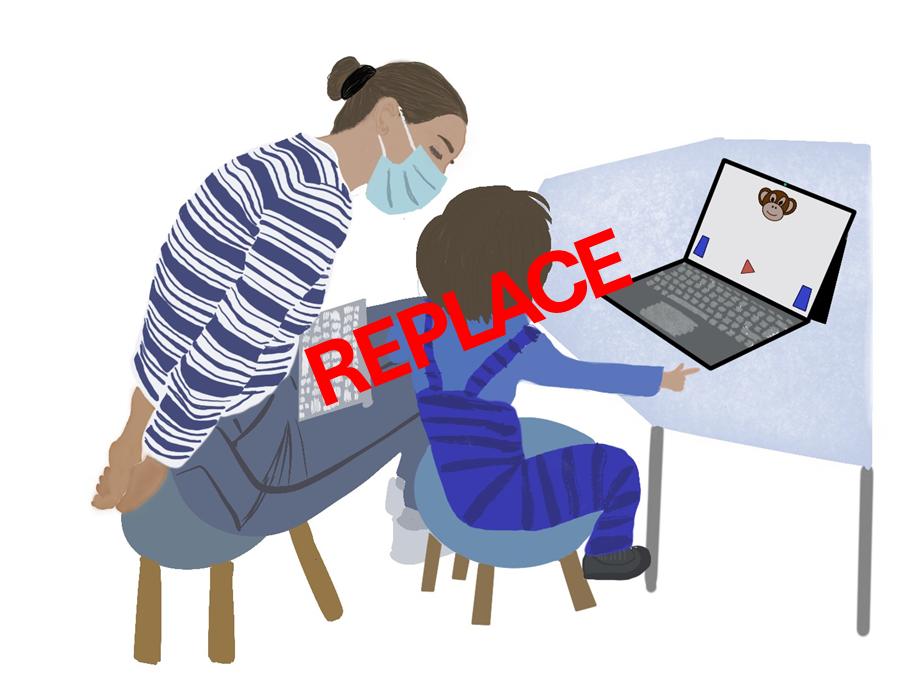
\includegraphics{./illustrations/Symlit_Rep_Setup} 

}

\caption{Illustration of setup.}\label{fig:pilot1illustration}
\end{figure}

\subsection{Materials}\label{materials}

Description of cues and targets and maybe how they were created. For an illustration of the stimuli and example presentations, please see supplementary materials sections XX and XX.

\subsection{Coding and Reliability}\label{coding-and-reliability}

Lorem ipsum dolor sit amet, consetetur sadipscing elitr, sed diam nonumy eirmod tempor invidunt ut labore et dolore magna aliquyam erat, sed diam voluptua. At vero eos et accusam et justo duo dolores et ea rebum. Stet clita kasd gubergren, no sea takimata sanctus est Lorem ipsum dolor sit amet. Lorem ipsum dolor sit amet, consetetur sadipscing elitr, sed diam nonumy eirmod tempor invidunt ut labore et dolore magna aliquyam erat, sed diam voluptua. At vero eos et accusam et justo duo dolores et ea rebum. Stet clita kasd gubergren, no sea takimata sanctus est Lorem ipsum dolor sit amet.

\subsection{Data analysis}\label{data-analysis}

For our main analyses, we used logistic Bayesian generalized linear mixed models (GLMM) to fit children's responses (0/1) as a function of their absolute age in days, task (arrow, marker) and an interaction between trial and task. We used default priors and included trial and sex as fixed effects to be controlled for. Trial number was added as a random slope within subject. The full model notation was 'correct \textasciitilde{} task*z.age +z.trial +z.sex +(z.trial\textbar id)'.

The analysis models participants binary choices to predict the probability of children interpreting the cues correctly and model how this probability will change as a function of their absolute age in days. In order to evaluate the relevance of age and task type for children's performance, we compared a full model as specified above with a reduced model lacking the interaction of age and task by using WAIC scores and weights (McElreath, 2016). Furthermore, we inspected the model estimates for the different predictors (including their 95\% Credible Interval (CrI)). To answer our main research question of when children perform above chance in a task, we use the model to predict the developmental trajectory (with 95\% CrI) for each task type. The criterion for settling when children perform above chance is the point at which the 95\% CrI for a particular trajectory does no longer overlap with a midline demarcating the 50\% chance level.

To further explore our data, we also binned participants in age-groups (three-, and four-year-olds). To test whether group-level performance was above chance in all experimental groups, we used two-tailed one-sample t-tests with the chance level set to .5. We provide Cohen's d as a standardized effect size for significance testing (computed via the function \texttt{cohensD}). Additionally, each participant's data was also submitted to a binomial test to determine whether their performance was above chance on an individual level.

All analyses were run in R (R Core Team, 2022). Bayesian models were run in Stan (\url{http://mc-stan.org/}) and implemented via the function brm of the package brms (Bürkner, 2017). Data and manuscript were prepared using the papaja and tidyverse packages Wickham (2017).

\section{Discussion}\label{discussion}

Lorem ipsum dolor sit amet, consetetur sadipscing elitr, sed diam nonumy eirmod tempor invidunt ut labore et dolore magna aliquyam erat, sed diam voluptua. At vero eos et accusam et justo duo dolores et ea rebum. Stet clita kasd gubergren, no sea takimata sanctus est Lorem ipsum dolor sit amet. Lorem ipsum dolor sit amet, consetetur sadipscing elitr, sed diam nonumy eirmod tempor invidunt ut labore et dolore magna aliquyam erat, sed diam voluptua. At vero eos et accusam et justo duo dolores et ea rebum. Stet clita kasd gubergren, no sea takimata sanctus est Lorem ipsum dolor sit amet.

\newpage

\section{References}\label{references}

\begingroup
\setlength{\parindent}{-0.5in}
\setlength{\leftskip}{0.5in}

\phantomsection\label{refs}
\begin{CSLReferences}{1}{0}
\bibitem[\citeproctext]{ref-R-papaja}
Aust, F., \& Barth, M. (2022). \emph{{papaja}: {Prepare} reproducible {APA} journal articles with {R Markdown}}. Retrieved from \url{https://github.com/crsh/papaja}

\bibitem[\citeproctext]{ref-bohn2019young}
Bohn, M., Kachel, G., \& Tomasello, M. (2019). Young children spontaneously recreate core properties of language in a new modality. \emph{Proceedings of the National Academy of Sciences}, \emph{116}(51), 26072--26077.

\bibitem[\citeproctext]{ref-R-base}
R Core Team. (2022). \emph{R: A language and environment for statistical computing}. Vienna, Austria: R Foundation for Statistical Computing. Retrieved from \url{https://www.R-project.org/}

\bibitem[\citeproctext]{ref-simmons201221}
Simmons, J. P., Nelson, L. D., \& Simonsohn, U. (2012). A 21 word solution. \emph{Available at SSRN 2160588}.

\bibitem[\citeproctext]{ref-R-tidyverse}
Wickham, H. (2017). \emph{Tidyverse: Easily install and load the 'tidyverse'}. Retrieved from \url{https://CRAN.R-project.org/package=tidyverse}

\end{CSLReferences}

\endgroup


\end{document}
